\documentclass{beamer}
\mode<presentation>
%% \mode<handout>{\setbeamercolor{background canvas}{bg=black!5}}
\usetheme{CambridgeUS}
\usecolortheme{dolphin}

\usepackage{../bstyle}

\title[TDA with Real Data]{
TDA With Real Data: Un-Complicating Distance Computations
}
\author[B.\ Fasy]{Brittany Terese Fasy}
\institute[MSU]{Montana State University}
\date[2 April 2026]{2 April 2026\\
    Guest Lecture, Computational Topology\\
    University of Utah}

\begin{document}

\begin{frame}
\titlepage
\end{frame}

\frame{
    \frametitle{}

    \begin{block}{}
        \begin{itemize}
            \item Thanks for having me!
            \item \url{WinCompTop+subscribe@googlegroups.com}
        \end{itemize}
    \end{block}
}

\begin{frame}
  \frametitle{Collaborator Collage}
  \framesubtitle{Grants: NSF DMS 1664858, NSF CCF 2046730,  NSF CBET 2152737}

  \begin{columns}

  \column{.15\textwidth}
  \centering
  
\includegraphics[width=\textwidth]{people/comptag/alex}\\
  
\includegraphics[width=\textwidth]{people/comptag/anna}\\
  
\includegraphics[width=\textwidth]{people/comptag/ben}\\

  \column{.15\textwidth}
  \centering
  
\includegraphics[width=\textwidth]{people/comptag/binhai}\\
  
\includegraphics[width=\textwidth]{people/collab/brian}\\
  
\includegraphics[width=\textwidth]{people/collab/carola}\\

  \column{.15\textwidth}
  \centering
  
\includegraphics[width=\textwidth]{people/comptag/dave}\\
  
\includegraphics[width=\textwidth]{people/collab/demi}\\

  \column{.15\textwidth}
  \centering
  
\includegraphics[width=\textwidth]{people/comptag/jack}\\
  
\includegraphics[width=\textwidth]{people/collab/jessi}\\
  
\includegraphics[width=\textwidth]{people/collab/jisu}\\

  \column{.15\textwidth}
  \centering
  
\includegraphics[width=\textwidth]{people/comptag/sam}\\
  
\includegraphics[width=\textwidth]{people/collab/jqbrown}\\
    \end{columns}
\end{frame}

\section{Introduction}

\frame{
\frametitle{Why Topological Data Analysis?}
\framesubtitle{~}
\begin{block}{}
 Today, Data is high-dimensional, \onslide<2->{terabytes large,}
    \onslide<3->{\& present everywhere}
 \vspace{.2in}
 \begin{columns}
  \column{.32\textwidth}
   
\includegraphics[width=\textwidth,height=1.25in]{examples/stanford-reeb}%
   \\
   ---------------------\\
   \scriptsize{Nicolaua, Levine, and Carlsson, PNAS 2011}
   \column{.32\textwidth}
     \onslide<2->{
\includegraphics[width=\textwidth,height=1.25in]{gleason/slide}
   \\
   ---------------------\\
   \scriptsize{Collab.~with\\ Tulane University}
   }%
   \column{.32\textwidth}
   \onslide<3->{
   \vspace{.2in} \\
   
\includegraphics[width=\textwidth]{roads/chicago-tracks}
   \vspace{.05in} \\
   ---------------------\\
   \scriptsize{Data available at www.mapconstruction.org}
   }
 \end{columns}
 \vspace{.2in}
    ... and needs to be summarized \& compared!

\end{block}
}



%%%%%%%%%%%%%%%%%%%%%%%%%%%%%%%%%%%%%%%%%%%%%%%%%%%%%%%%%
%%%%%%%%%%%%%%%%%%%%%%%%%%%%%%%%%%%%%%%%%%%%%%%%%%%%%%%%%
\section{Motivating Example}
%%%%%%%%%%%%%%%%%%%%%%%%%%%%%%%%%%%%%%%%%%%%%%%%%%%%%%%%%
%%%%%%%%%%%%%%%%%%%%%%%%%%%%%%%%%%%%%%%%%%%%%%%%%%%%%%%%%

%%%%%%%%%%%%%%%%%%%%%%%%%%%%%%%%%%%%%%%%%%%%%%%%%%%%%%%%%
\begin{frame}
\frametitle{Prostate Cancer}
\framesubtitle{The Question is \emph{Will He Outlive It?}}

    \begin{block}{}
        \begin{itemize}
            \item $1.5$M cases diagnosed per year worldwide.
            \item One is seven men will be diagnosed.
            \item Treatments: surgery, chemo, radiation, harmone therapy.
            \item Either slowly-growing  and benign or fast-growing
                and dangerous.
            \item Surgery / radiation benefits questionable for SG/B.
            \item Surgery / radiation side effects not desirable.
            \item ... therefore, active surveillance.
        \end{itemize}
    \end{block}

\end{frame}
%%%%%%%%%%%%%%%%%%%%%%%%%%%%%%%%%%%%%%%%%%%%%%%%%%%%%%%%%

%%%%%%%%%%%%%%%%%%%%%%%%%%%%%%%%%%%%%%%%%%%%%%%%%%%%%%%%%
\begin{frame}
\frametitle{Prostate Cancer}
\framesubtitle{Diagnosis}

\centering
    \only<1->{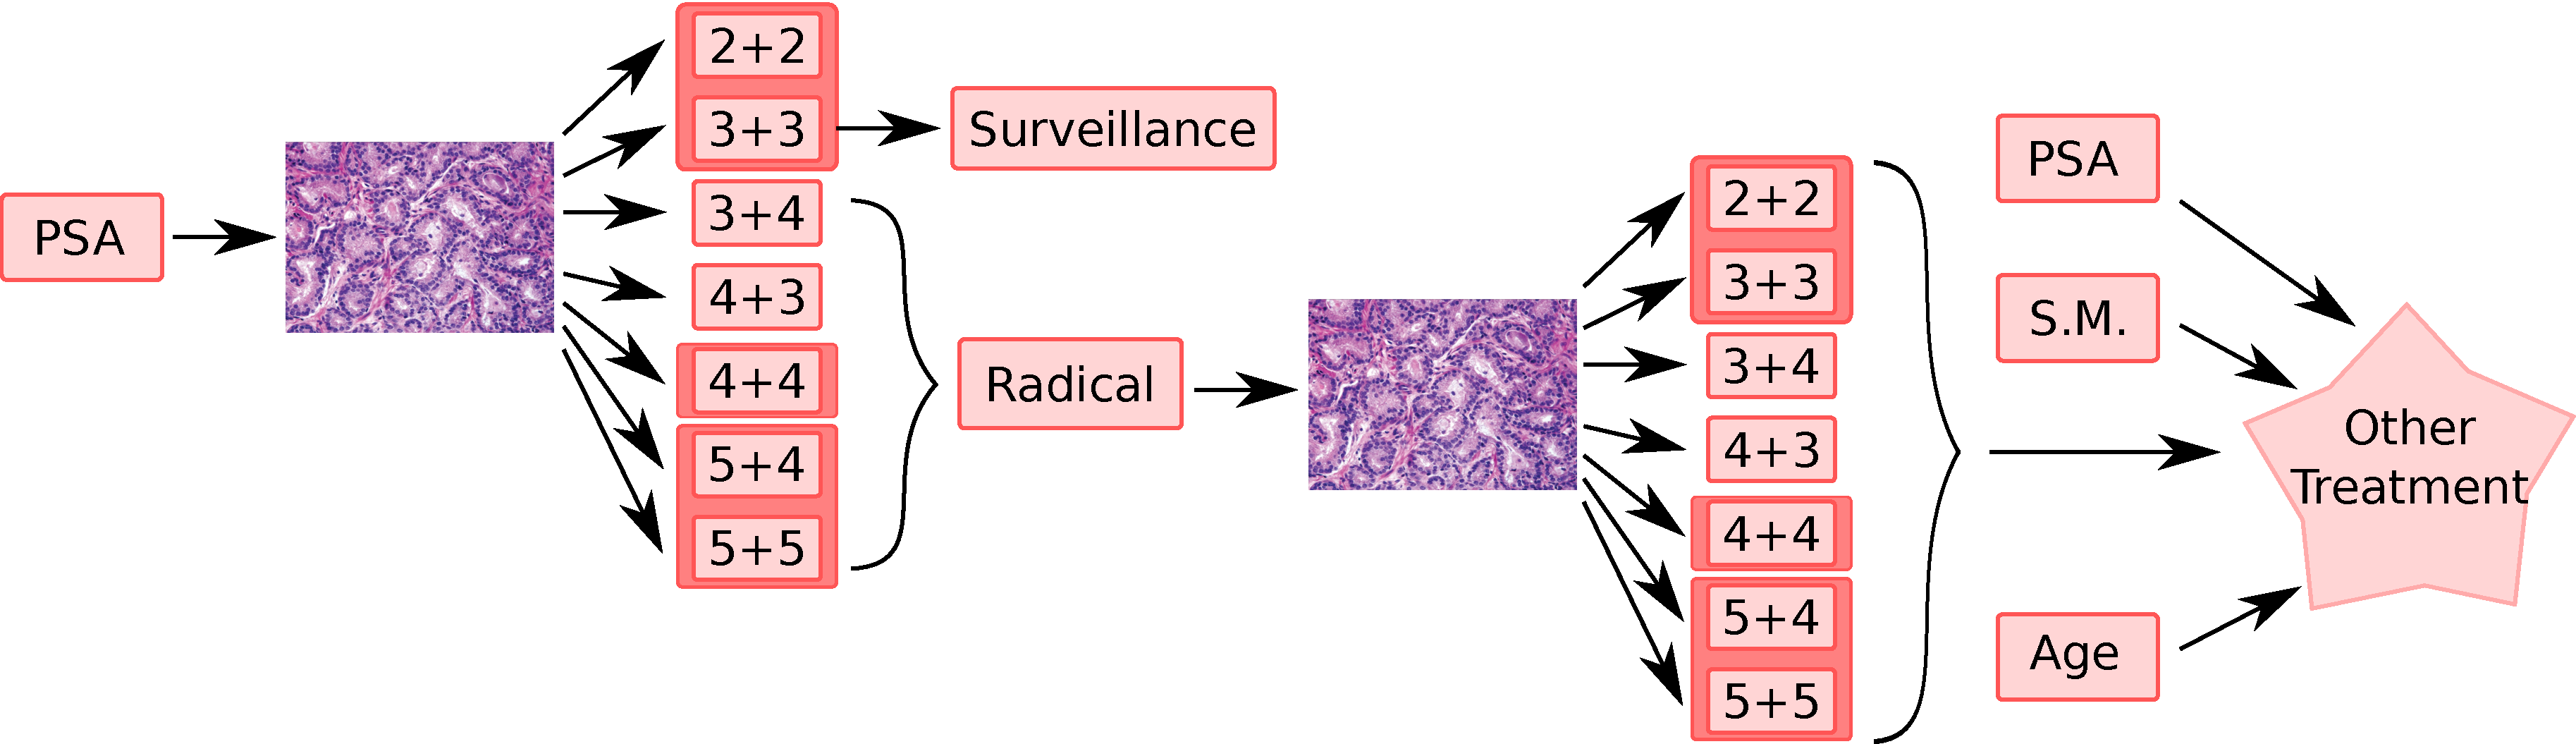
\includegraphics[width=\textwidth]{../figs/gleason/gleason-process}}

\end{frame}
%%%%%%%%%%%%%%%%%%%%%%%%%%%%%%%%%%%%%%%%%%%%%%%%%%%%%%%%%

%%%%%%%%%%%%%%%%%%%%%%%%%%%%%%%%%%%%%%%%%%%%%%%%%%%%%%%%%
\begin{frame}
\frametitle{Gleason Grading}
\framesubtitle{~}

    \begin{columns}
        \column{.45\textwidth}
        \centering
        \only<1>{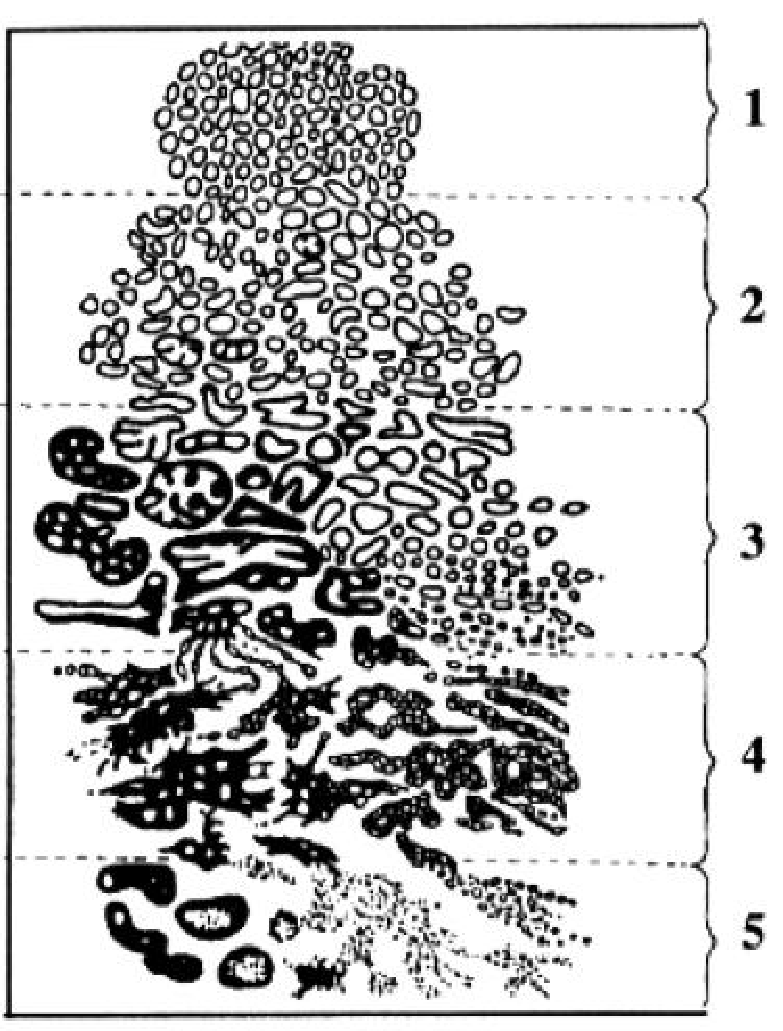
\includegraphics[height=2in]{../figs/gleason/gleason-old}}
        \only<2->{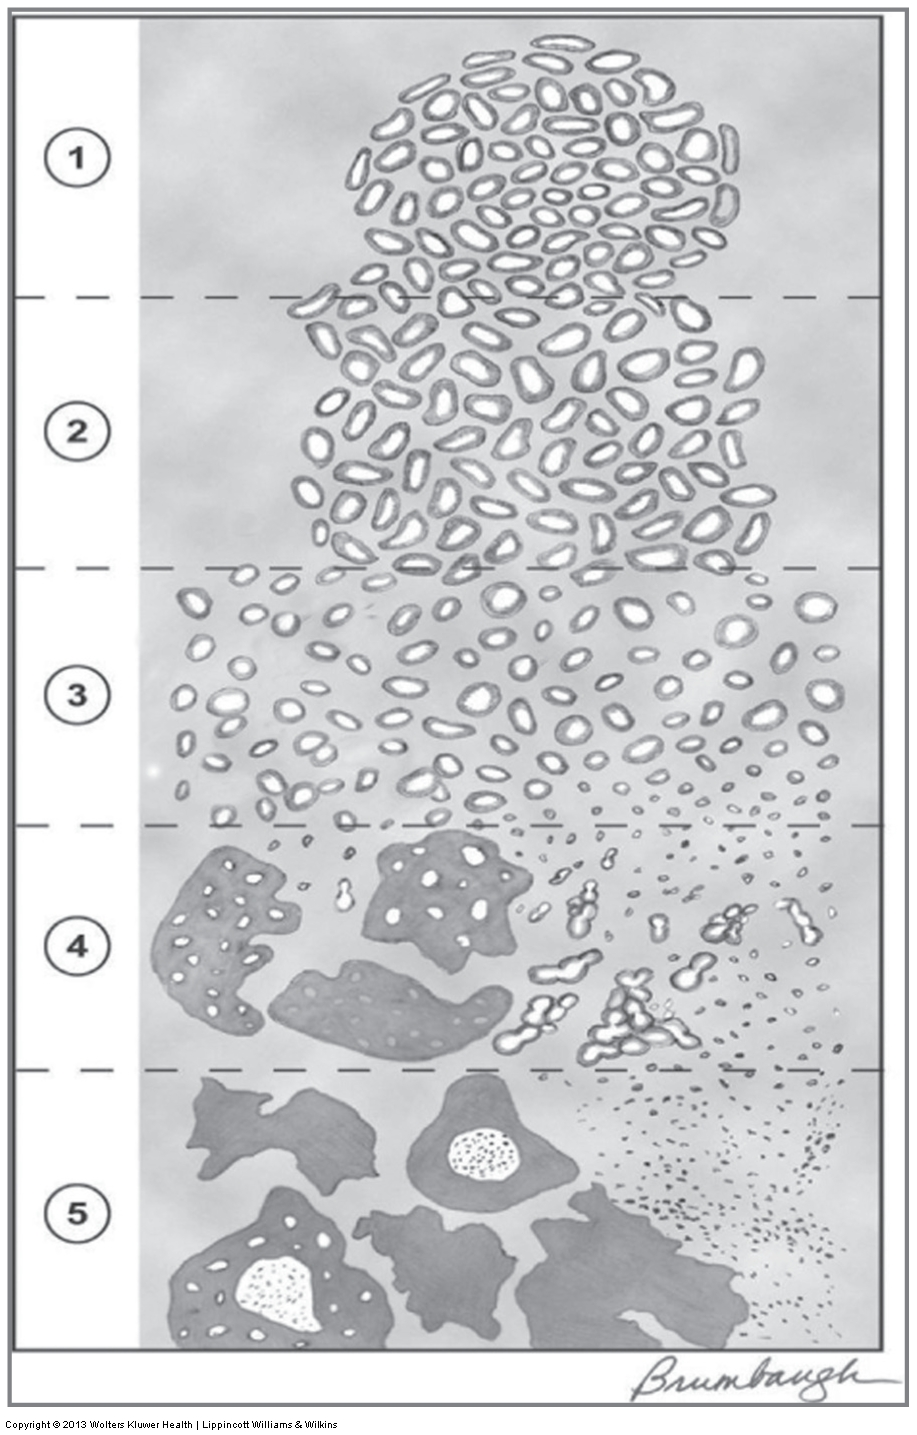
\includegraphics[height=2in]{../figs/gleason/gleason-new}}
        \column{.45\textwidth}
        \begin{block}{}
            \hangindent=1.5cm
            \hangafter=1
            \noindent
            Grade 1: well-defined, nicely packed

            \hangindent=1.5cm
            \hangafter=1
            \noindent
            Grade 2: larger, more tissue,  less uniform


            \hangindent=1.5cm
            \hangafter=1
            \noindent
            Grade 3: less defined glands%
            \only<1>{, some cribriform}

            \hangindent=1.5cm
            \hangafter=1
            \noindent
            Grade 4: fused glands, open lumens%
            \only<2->{, cribriform}

            \hangindent=1.5cm
            \hangafter=1
            \noindent
            Grade 5: no glandular definition, sheets of cells
        \end{block}
    \end{columns}
    \only<1>{\footnotetext{
        Donald Gleason, 1966, image from \emph{The Gleason Grading System: A Complete
        Guide for Pathologist and Clinicians} by Eppstein}}
    \only<2>{\footnotetext{
        2005 Consensus, image from \emph{The Gleason Grading System: A Complete
        Guide for Pathologist and Clinicians} by Eppstein}}

\end{frame}
%%%%%%%%%%%%%%%%%%%%%%%%%%%%%%%%%%%%%%%%%%%%%%%%%%%%%%%%%

%%%%%%%%%%%%%%%%%%%%%%%%%%%%%%%%%%%%%%%%%%%%%%%%%%%%%%%%%
\begin{frame}
\frametitle{Prostate Cancer}
\framesubtitle{Diagnosis}

\centering
    \onslide<1->{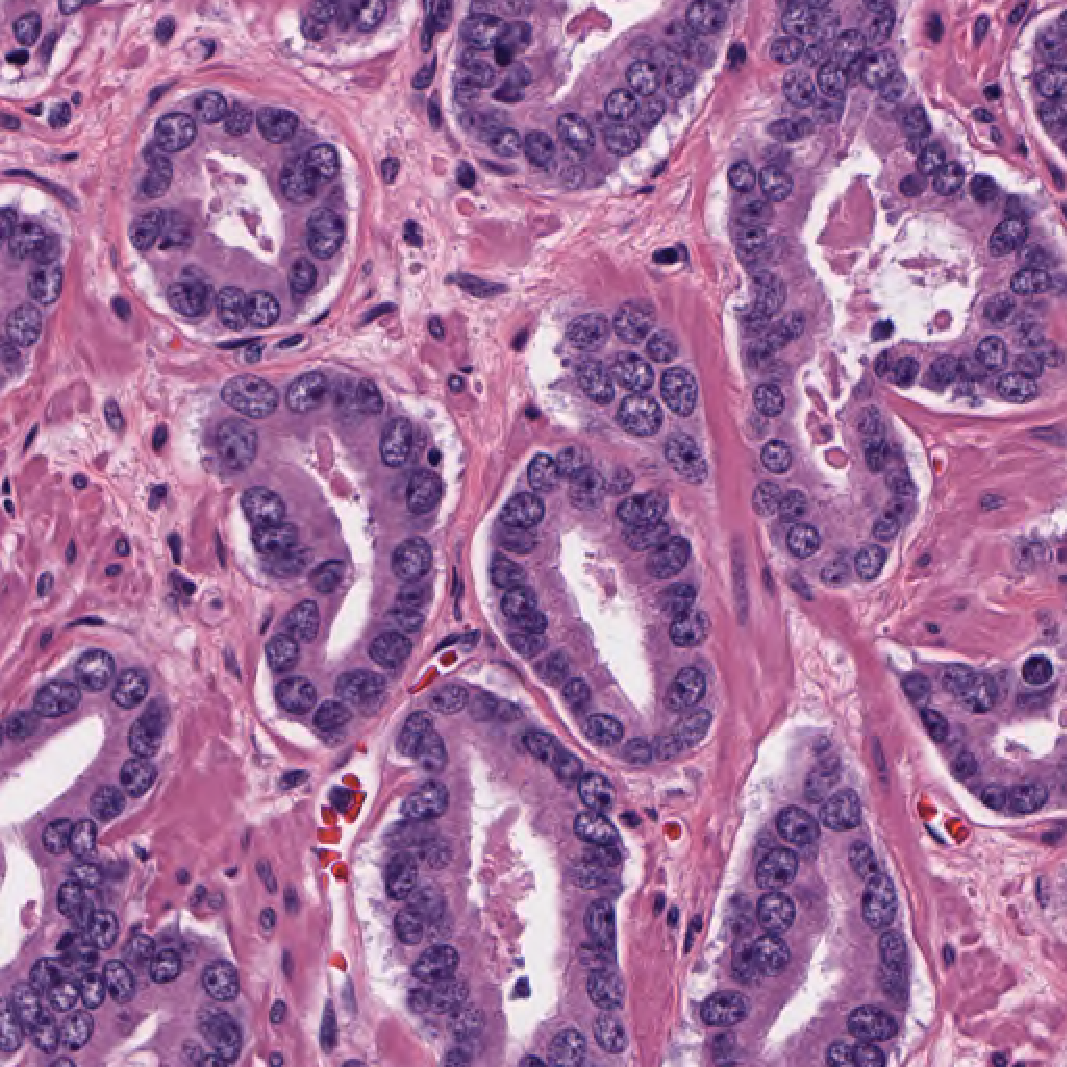
\includegraphics[width=.45\textwidth]{../figs/gleason/gleason3}}
    \quad
    \onslide<2->{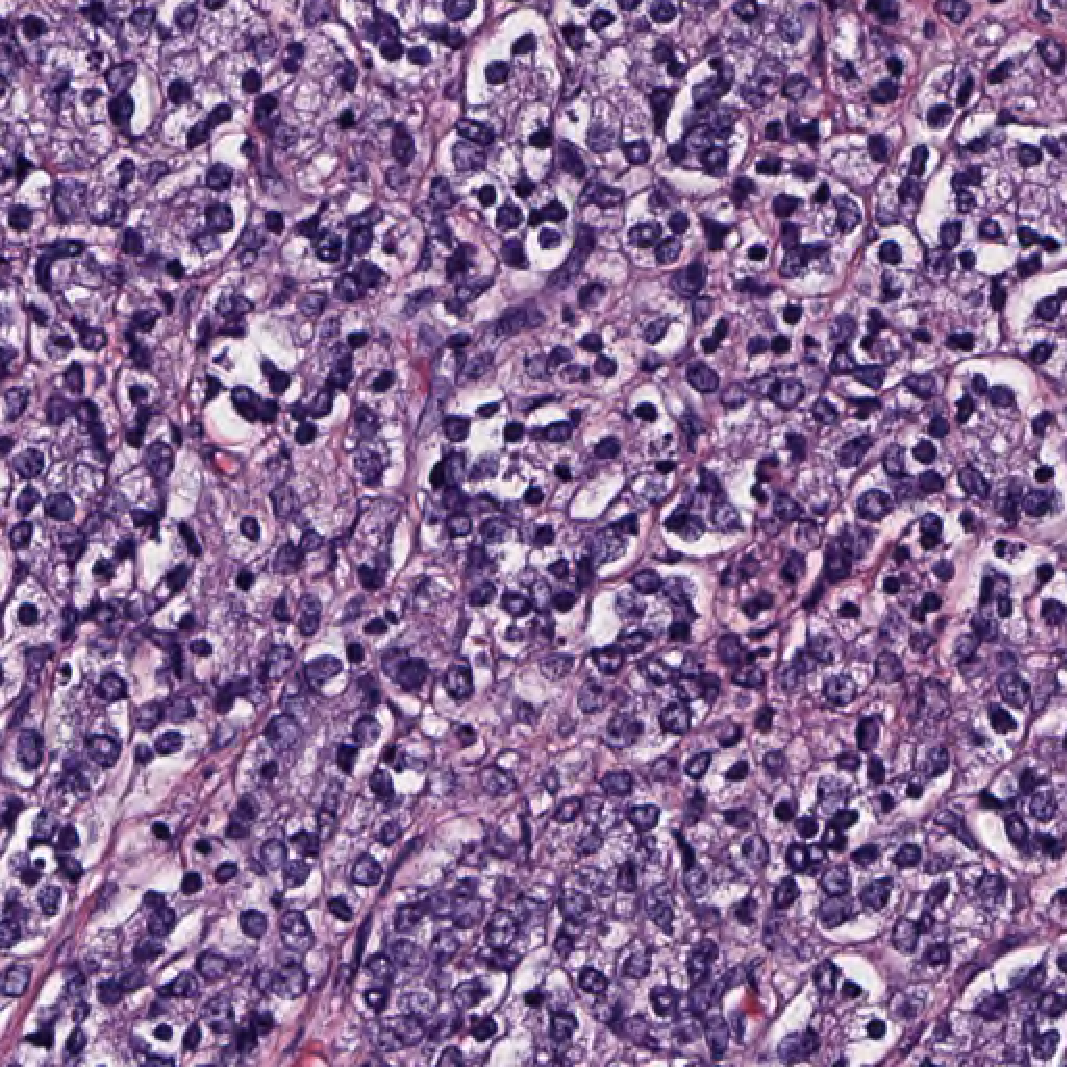
\includegraphics[width=.45\textwidth]{../figs/gleason/gleason5}}
\end{frame}
%%%%%%%%%%%%%%%%%%%%%%%%%%%%%%%%%%%%%%%%%%%%%%%%%%%%%%%%%

\frame<1->[label=compareGlands]{
\frametitle{}

\begin{block}{}
\centering
 \only<1>{
\includegraphics[width=.7\textwidth]{gleason/compare-0}}%
 \only<2>{
\includegraphics[width=.7\textwidth]{topology/inference-compare-1}}%
 \only<3->{
\includegraphics[width=.7\textwidth]{topology/inference-compare-2}}%
\end{block}

}

\begin{frame}
    \frametitle{Real Data}
    \framesubtitle{P.\ Lawson, J.Q.\ Brown, BTF, C.\ Wenk, A.\ Scholl, Sci
    Reports 9, 2019.}

    \begin{block}{}
        \centering
        \only<1>{
\includegraphics[height=2in]{gleason/tsne_fig_hist}}
    \end{block}
\end{frame}

\section{Persistence Diagrams}

\frame{
    \frametitle{... But}

    \pause
    \begin{block}{Real Data is Large and Messy}
        \centering
        \only<1->{
\includegraphics[width=.7\textwidth]{gleason/roi}}%
    \end{block}

    \pause
    \begin{block}{}
        And Diagram Space is Ugly ...
    \end{block}
}

\frame{
    \frametitle{Distances Between Diagrams}

    \centering
    \only<1>{
\includegraphics[height=2in]{pd-search/diagram-empty}}%
    \only<2>{
\includegraphics[height=2in]{pd-search/diagram-matching}}%
    \only<3>{
\includegraphics[height=2in]{pd-search/diagram-partialmatch}}%
    \only<4->{
\includegraphics[height=2in]{pd-search/diagram-todiag}}%

    \begin{block}{}
        $$
        d_q(D_1,D_2) := \min_{\mathcal{M}} \left(
            {\only<3>{\color{red}} \sum_{(a,b)\in \mathcal{M}} ||a-b||_{\infty}^q} +
            {\only<4->{\color{blue}} \frac{1}{2^{q-1}} \sum_{a \in \mathcal{M}^c} |a_x-a_y|^q}
        \right)^{1/q}
        $$
    \end{block}

}

\frame<1>{
    \frametitle{Alternate Distances Between Diagrams}

    \begin{columns}
        \column{.45\textwidth}
        \centering
        
\includegraphics[width=\textwidth]{gleason/MDSlarge}
    \column{.55\textwidth}
    \begin{block}{}
        \begin{itemize}
            \item Wasserstein $d_q$.
            \item Bottleneck / interleaving~$d_{\infty}$.
            \item Erosion distance. \pause
            \item (Distances in function space.)
        \end{itemize}
    \end{block}
    \end{columns}
}

\frame{
    \frametitle{Summarizing with Averaging}

    \begin{columns}
        \column{.45\textwidth}
            \begin{block}{Data}
                $\mathcal{D} \subset \mathbb{D}_M^m$
            \end{block}
            \pause
            \begin{block}{\checkmark Fr\'echet Variance defined!}
                Let $D \in \mathbb{D}_M^m$ and $\mathcal{D} \subset
                \mathbb{D}_M^m$.
                $$ V_p(D, \mathcal{D}) := \sum_{A \in \mathcal{D}} d_p^2(A,D)  $$
            \end{block}
            \pause
            \begin{block}{... But Nonunique Means}
                $$ \mu_p(\mathcal{D}) := \argmin_{D \in \mathcal{D}} V_p(D,\mathcal{D} ) $$
            \end{block}
        \column{.45\textwidth}
        \begin{block}{}
            \centering
            \only<3>{
\includegraphics[height=2in]{stat/frechet-mean}}%
            \only<4>{
\includegraphics[height=2in]{stat/frechet-mean1}}%
            \only<5->{
\includegraphics[height=2in]{stat/frechet-mean2}}%
        \end{block}
        %
        \footnotesize
        \begin{block}{References}
            \begin{itemize}
                \item Turner et al., DCG 2014
                \item Munch et al., EJS 2015
            \end{itemize}
        \end{block}
    \end{columns}
}

\frame{
    \frametitle{The Metric Space $(\mathcal{D}_M^m, d_{\infty})$}

    \begin{columns}
        \column{.45\textwidth}
        \pause
        \begin{block}{As a Set}
            $(M,m)$-bounded diagrams:\pause
            \begin{itemize}
                \item $M$, maximum absolute values of finite coordinates\pause
                \item $m$, upper bound for size \pause
            \end{itemize}
        \end{block}
        \column{.45\textwidth}
        \begin{block}{As a Space}
            The metric topology \pause
        \end{block}
        \begin{block}{Theorem, ArXiv 1812.11257}
            Infinite doubling dimension!
        \end{block}
    \end{columns}
}

\frame{
    \begin{block}{}
        ... so, what can we do with persistence diagrams?
    \end{block}
}

\frame{
    \begin{block}{Working with Diagrams Directly:}
    Near Neighbor Search
    \end{block}
}

\frame{
    \frametitle{Nearest Neighbor Search}
\begin{block}{}
    \centering
    \onslide<3->{
\includegraphics[height=2in]{pd-search/dgm-query}}
    \quad\quad
    \only<1>{
\includegraphics[height=2in]{pd-search/dgm-songs}}%
    \only<2->{
\includegraphics[height=2in]{pd-search/dgm-set}}%
\end{block}

}


%new version first, then old
\frame{
    \frametitle{Problem Setup}

    \begin{columns}
        \column{.45\textwidth}
        \begin{block}{}
            \centering
            \onslide<3->{
\includegraphics[height=1in]{pd-search/dgm-query}}
            \quad\quad
            \only<1>{
\includegraphics[height=1in]{pd-search/dgm-songs}}%
            \only<2->{
\includegraphics[height=1in]{pd-search/dgm-set}}%
        \end{block}

        \column{.45\textwidth}
        \begin{block}{}
            \begin{itemize}
                \item \only<2->{\st}{Given data} \pause
                \item Given a set of diagrams $\Gamma$ \pause
                \item and a query diagram $Q$ \pause
                \item Find $Q' \in \Gamma$ minimizing $$d_{\infty}(Q,Q')$$
            \end{itemize}
        \end{block}

    \end{columns}
}

\frame{
    \frametitle{A Tried and True Way}
    \onslide<2->{\framesubtitle{... in Nice Enough Spaces}}

    \begin{columns}
        \column{.45\textwidth}
            \only<1>{
\includegraphics[height=2in]{pd-search/nice-search-0}}%
            \only<2>{
\includegraphics[height=2in]{pd-search/nice-search-1}}%
            \only<3>{
\includegraphics[height=2in]{pd-search/nice-search-2}}%
            \only<4>{
\includegraphics[height=2in]{pd-search/nice-search-3}}%
            \only<5>{
\includegraphics[height=2in]{pd-search/nice-search-4}}%
            \only<6>{
\includegraphics[height=2in]{pd-search/nice-search-5}}%
            \only<7>{
\includegraphics[height=2in]{pd-search/nice-search-6}}%
            \only<8>{
\includegraphics[height=2in]{pd-search/nice-search-7}}%
            \only<9>{
\includegraphics[height=2in]{pd-search/nice-search-8}}%
            \only<10>{
\includegraphics[height=2in]{pd-search/nice-search-9}}%
            \only<11>{
\includegraphics[height=2in]{pd-search/nice-search-10}}%
            \only<12->{
\includegraphics[height=2in]{pd-search/nice-search-found}}%
        \column{.45\textwidth}
        \onslide<13->{
        \begin{block}{}
            Exponential in the DD.\\
            \onslide<14->{
                Recall: $\mathbb{D}_M^m$ has infinite DD.}\\
            \onslide<15->{$\implies$ not for PersDgms!\\ }
        \end{block}
        \onslide<16->{
            \begin{block}{}
                    In practice: just linear search.\\
            \end{block}
        }
    }
    \end{columns}
}



\frame{
    \frametitle{Near Neighbor Search}

\begin{columns}
    \column{.5\textwidth}
   \begin{block}{Nearest Neighbor}
       Given: $\mathcal{D}$ and $Q$, find:
        $$ {\color{blue} Q_{NN}} := \arg\min_{Q' \in \mathcal{D}} d(Q,Q').$$
    \end{block}
    \pause
    \begin{block}{Approximate Nearest Neighbor}
        Find some $\widetilde{Q} \in \mathcal{D}$ such that:
        $$d({\color{blue} Q_{NN}},Q) \leq d(\widetilde{Q},Q)
        \leq {\color{red} c}\cdot d({\color{blue} Q_{NN}},Q)$$
    \end{block}

    \column{.45\textwidth}
    \pause
      \begin{block}{Considerations}
          \begin{itemize}
              \item Want: $ {\color{red} c}$ small
              \pause \item Query time
              \pause \item Size of data structure
              \pause \item Precomputation time
          \end{itemize}
      \end{block}

\end{columns}
}

\section{Searching for Near Neighbors}

\frame{
     \frametitle{Related Work [Driemel and Silvestri, SoCG 2017]}

     \begin{block}{Locality Sensitive Hashing of Curves}
         
\includegraphics[width=\textwidth]{pd-search/driemel.png}
     \end{block}
}

\frame[label=firstAttempt]{
     \frametitle{First Attempt}
     \framesubtitle{Inspired by Locality Sensitive Hashing (LSH)}

     \begin{block}{Probabilistic Near Neighbor}
         With high probability, we find a near-neighbor using
         \begin{itemize}
             \item $O(2^{12m} m \log n + 2^{12m} \log^2 n)$ time.
             \item $O(2^{12m} n \log n + nm)$ space.
             \item $O(UGLY)$ precomputation.
             \item Approximation factor: $ {\color{red} c} =8 \sqrt{2} \approx 11.3$.
         \end{itemize}
     \end{block}
 }



\frame{
    \frametitle{Locality Sensitive Hashing}

    \begin{block}{}
        \centering
        Hashing $\implies$ probabilistic\\ \pause
        What if ... we lose the randomness?
    \end{block}
}


\frame[label=dsNalgo]{
    \frametitle{Overview of Data Structure and Algorithm}
    \begin{columns}
        \column{.45\textwidth}
        \begin{block}{Data Structure / Precomputation}
            \begin{itemize}
                \item $\tau$ levels.
                \item Increase level, increase resolution.
                \item At each level $i$,
                    \begin{itemize}
                        \item $O(5^m)$ snap-roundings of each $P \in \mathcal{D}$.
                        \item Compute key for each.
                        \item Sort keys.
                    \end{itemize}
            \end{itemize}
        \end{block}



        \column{.5\textwidth}
        \pause
        \begin{block}{Algorithm}
            \begin{enumerate}
                \item Binary search levels to find lowest collision. At each level $i$:
                    \begin{itemize}
                        \item Compute key $\kappa_i(Q)$.
                        \item Search level for collision.
                        \item If collides, down. Else, stop.
                    \end{itemize}
                \item Choose any diagram in last bin.
            \end{enumerate}
        \end{block}
    \end{columns}
}

\frame<8>[label=dgmsearch]{
    \frametitle{Snap-Rounding Persistence Diagram}
    \onslide<3->{\frametitle{Search for Near Persistence Diagram}}

    \centering
    % \only<1>{
    %     \includegraphics[width=\textwidth]{pd-search/example-diagrams}}%
    % \only<2>{
    %     \includegraphics[width=\textwidth]{pd-search/example-snapping}}%
    \only<3>{
        
\includegraphics[width=\textwidth]{pd-search/data-structure-level-1}}%
    \only<4>{
        
\includegraphics[width=\textwidth]{pd-search/data-structure-level-2}}%
    \only<5>{
        
\includegraphics[width=\textwidth]{pd-search/data-structure-level3-nox}}%
    \only<6>{
        
\includegraphics[width=\textwidth]{pd-search/data-structure-level-3}}%
    \only<7>{
        
\includegraphics[width=\textwidth]{pd-search/data-structure-level-4}}%
    \only<8->{
        
\includegraphics[height=3in]{pd-search/data-structure}}%
}



\frame<2->{
    \frametitle{Compute Keys}

    \begin{block}{}
        \begin{columns}
            \column{.5\textwidth}
            \begin{itemize}
                \item $P$ is a point cloud.
                \item Consider $\eta \times \eta$ square lattice $\mathcal{L}$.
                \item Snap points in $P$ to $\mathcal{L}$.
                \item Compute count vector.
            \end{itemize}

            \column{.5\textwidth}
            \centering
            \only<2>{
\includegraphics[height=2in]{pd-search/example-ingridcell}}%
            \only<3>{
\includegraphics[height=2in]{pd-search/example-allsnap}}%
            \only<4>{
\includegraphics[height=2in]{pd-search/example-vec1}}%
            \only<5>{
\includegraphics[height=2in]{pd-search/example-vec2}}%
            \only<6>{
\includegraphics[height=2in]{pd-search/example-vec3}}%
            \only<7>{
\includegraphics[height=2in]{pd-search/example-vec4}}%
            \\
            \onslide<4->{$\langle
            \only<4>{1,0,0,0,0,0,0,0,1}
            \only<5>{0,1,0,0,0,0,0,0,1}
            \only<6>{0,0,0,0,2,0,0,0,0}
            \only<7>{0,0,0,0,1,0,0,0,1}
            \rangle$}
        \end{columns}
        \end{block}
    }


\frame{
    \frametitle{... What About the Diagonal?}

    \begin{block}{}
        \centering
        \only<1>{
\includegraphics[height=2.5in]{pd-search/diagram-matching}}%
        \only<2>{
\includegraphics[height=2.5in]{pd-search/diagram-del}}%
        \only<3>{
\includegraphics[height=2.5in]{pd-search/diagram-delmore}}%
        \only<4->{
\includegraphics[height=2.5in]{pd-search/diagram-delpts}}%
    \end{block}
}

\frame{
    \frametitle{Refining Grid}
    \begin{block}{}
        \centering
        
\includegraphics[height=2.5in]{pd-search/multiple-resolution}
    \end{block}
}


\againframe<3->{dgmsearch}




\frame<1->[label=dsproperties]{
    \frametitle{Properties of the Data Structure for $\mathcal{D}$}

    \begin{columns}
        \column{.45\textwidth}
         \begin{block}{Collision}
             If $d(P,Q) \leq \frac{1}{2}\delta_i$, then
             $Q$ collides with $P$ at level $i$.
         \end{block}
         \column{.45\textwidth}
         \onslide<2->{
             \begin{block}{No Collision}
                 If $d(P,Q) > \frac{3}{2}\delta_i$, then
                 $Q$ does not collide with $P$ at level $i$.
             \end{block}


    }
    \end{columns}

    \onslide<3->{
    \begin{block}{}
        \begin{itemize}
            \onslide<4->{ \item Notice that this is nearly an iff statement.}
            \onslide<5->{ \item Do we have a heirarchical collision or is
                there a gap?}
        \end{itemize}

        \centering
        \only<1-4>{
            
\includegraphics[height=0.5in]{pd-search/gap-i}}%
        \only<5->{
            
\includegraphics[height=0.5in]{pd-search/gap}}%

    \end{block}}
}

\frame<1-4>[label=hcl]{
    \frametitle{Hierarchical Collision Lemma}

    \begin{block}{Hierarchical Collision Lemma}
        If \only<1-4>{set} $Q$ collides with $P \in \mathcal{D}$ at level $j$, then
        $Q$ collides with $P$ for all $i \leq j$.
    \end{block}

    \onslide<2-4,6-8>{
    \begin{block}{Proof}
        Collision at level $j$ $\implies$ matching with cost $\leq
        \frac{3}{2}\delta_i$
        \onslide<4,8>{$\implies$ collision at $i$.}

        \centering
        \only<1-2>{
\includegraphics[height=1.5in]{pd-search/hcl-ptcloud-i}}%
        \only<3>{
\includegraphics[height=1.5in]{pd-search/hcl-ptcloud-lower-old}}%
        \only<4>{
\includegraphics[height=1.5in]{pd-search/hcl-ptcloud-lower}}%
        \only<5-6>{
\includegraphics[height=1.5in]{pd-search/hcl-dgm-i}}%
        \only<7>{
\includegraphics[height=1.5in]{pd-search/hcl-dgm-lower-old}}%
        \only<8>{
\includegraphics[height=1.5in]{pd-search/hcl-dgm-lower}}%
    \end{block}
    }
}



\againframe<5->{hcl}


\againframe{firstAttempt}
\frame[label=results]{
    \frametitle{Our Result}
    \framesubtitle{ArXiv 1812.11257}

    \begin{block}{Deterministic Near Neighbor}
        We find a near-neighbor using
        \begin{itemize}
            \item $O((m \log n + m^2)\log \tau)$ time.
            \item $O(\tau n5^m)$ space.
            \item $O(\tau nm 5^m \log{n})$ precomputation.
            \item Approximation factor: $  {\color{red} c}=6$.
        \end{itemize}
    \end{block}

}

\section{More Descriptors}

\frame{
    \begin{block}{}
       \centering
        That's nice, but ... \pause
        what else can we do?
    \end{block}
}

\frame{
    \frametitle{Transform to `Nicer' Spaces}

    \begin{block}{}
        \centering
        \only<1>{
\includegraphics[height=2.5in]{pd-search/dgm-set}}%
        \only<2->{
\includegraphics[height=2.5in]{pd-search/dgm-to-fcns}}%
    \end{block}
}

\frame{
    \frametitle{Some Other Spaces ...}

    \begin{columns}
        \column{.32\textwidth}
        \begin{block}{Diagram}
            \centering
            {
\includegraphics[height=.85in]{stat/persistence-imagedgm}}%
        \end{block}
        \pause
        \begin{block}{Landscapes}
            \centering
            {
\includegraphics[height=.85in]{stat/persistence-all-landscapes}}%
        \end{block}
        \column{.32\textwidth}
        \pause
        \begin{block}{Images}
            \centering
            {
\includegraphics[height=.85in]{stat/persistence-image}}%
        \end{block}
        \pause
        \begin{block}{Silhouette}
            \centering
            {
\includegraphics[height=.85in]{stat/persistence-silhouette}}%
        \end{block}

        \column{.32\textwidth}
        \pause
        \begin{block}{Betti Function}
            \centering
            {
\includegraphics[height=.85in]{stat/persistence-betti}}%
        \end{block}
        \pause
        \begin{block}{Euler Char.~Fcn}
            \centering
            {
\includegraphics[height=.85in]{stat/persistence-ecc}}%
        \end{block}
    \end{columns}
}

\frame{
    \frametitle{Some References ...}

    \small

    \begin{enumerate}

        \item Fr\'echet Mean: Turner, K., Mileyko, Y., Mukherjee, S., \& Harer,
            J. (2014). Fréchet means for distributions of persistence diagrams.
            Discrete \& Computational Geometry, 52(1), 44-70.

        \item Images: Adams, Emerson, Kirby, Neville, Peterson,
            Shipman, Chepushtanova, Hansen, Motta, \& Ziegelmeier. (2017). Persistence images: A
            stable vector representation of persistent homology. Journal of
            Machine Learning Research, 18.

        \item Landscapes: Bubenik (2015). Statistical topological data analysis using
            persistence landscapes. J. Mach. Learn. Res., 16(1), 77-102.

        \item Silhouettes: Chazal, Fasy, Lecci, Rinaldo, \& Wasserman, (2014,
            June). Stochastic convergence of persistence landscapes and
            silhouettes. In Proc.\ 13th Annual Symposium on
            Computational Geometry (pp. 474-483).

        \item Functional Summaries: Berry, Chen, Cisewski-Kehe, \& Fasy. (2020).
            Functional summaries of persistence diagrams. Journal of Applied and
            Computational Topology, 4(2), 211-262.

    \end{enumerate}
}

\begin{frame}
    \frametitle{Silhouettes}
    \framesubtitle{Experimental Set-Up}

    \begin{block}{}
        \begin{itemize}
            \item Training data: $2$k `glands', $500$ of each type\footnote{
                    Gland and slide simulator will be released soon; email if
                    interested! Brown, Fasy, Fox, Shenfisch, Schupbach, and Quist.}\pause
            \item Distance / DTM filtration\pause
            \item Silhouette, $p=1$\pause
            \item Test set: $400$, with $100$ of each type
            \item knn classification, with $k=3$
        \end{itemize}
    \end{block}

\end{frame}

\begin{frame}<1->[label=simulated]
    \frametitle{Silhouettes}
    \framesubtitle{Results}

    \begin{block}{Berry et al. 2020}
        \centering
        \only<1>{
\includegraphics[height=2.25in]{gleason/sil-mds-input}}
        \only<2->{
\includegraphics[height=2.25in]{gleason/sil-mds}}
    \end{block}
\end{frame}


\frame{
    \begin{block}{}

        Still need faster distance computations ...

    \end{block}
}

\frame<1>[label=reveal]{
    \frametitle{Clustering}
    \begin{block}{}

        \centering
        \only<1>{
\includegraphics[height=2in]{pd-search/vis21-teaser-pre}}%
        \only<2->{
\includegraphics[height=2in]{pd-search/vis21-teaser}}%

    \end{block}
}

\frame{
    \frametitle{General Idea}

    \begin{block}{}
        \centering
        \only<1>{
\includegraphics[height=2.75in]{pd-search/vis21-overview-2dgmonly}}%
        \only<2>{
\includegraphics[height=2.75in]{pd-search/vis21-overview-2images}}%
        \only<3>{
\includegraphics[height=2.75in]{pd-search/vis21-overview-2ml}}%
        \only<4->{
\includegraphics[height=2.75in]{pd-search/vis21-overview}}%
    \end{block}
}

\frame{
    \frametitle{Training Architecture}

    \begin{block}{}
        \centering
        
\includegraphics[width=\textwidth]{pd-search/PD-BGAN}
    \end{block}
}

\frame{
    \frametitle{Related Work}
    \framesubtitle{Binary Generative Adversarial Networks for Image Retrieval by
    Song et al.}

    \begin{block}{}
        \centering
        
\includegraphics[height=2.5in]{pd-search/song-abstract}
    \end{block}
}


\frame{
    \frametitle{Hashing for PD Distances}

    \begin{block}{}
        \begin{itemize}
            \item Qin, Fasy, Wenk, Summa. A Domain-Oblivious Approach for Learning Concise
                Representations of Filtered Topological Spaces for Clustering.
                IEEE Vis 2021.
            \item Code: \url{https://osf.io/q58c3/}
        \end{itemize}
    \end{block}

}

\frame{
    \frametitle{Input to GANN}
    \begin{block}{}
        \centering
        
\includegraphics[height=2in]{pd-search/histogram}
    \end{block}
}


\frame{
    \frametitle{Quality of Clusters}

    \begin{columns}
        \column{.45\textwidth}
        \begin{block}{Variables}
        \begin{itemize}
            \item ${{n}\choose{2}}$ pairs of diagrams
            \item $C_1$ = clustering in $(\mathcal{D},d_1)$
            \item $C_2$ = our clustering \pause
            \item $A^+$ = agree, same cluster
            \item $D^{+,-}$ = disagree
            \item $D^{-,+}$ = disagree
        \end{itemize}
        \end{block}

        \pause
        \column{.45\textwidth}
        \begin{block}{Fowlkes--Mallows Score (FMS)}
            $$ S = \frac{A^+}{\sqrt{(A^++D^{-,+})(A^++D^{+,-})}} $$
            \pause
            \begin{itemize}
                \item $S \in [0,1]$
                \item $S=1$ iff identical clusters
            \end{itemize}
        \end{block}
    \end{columns}
}

\frame[label=realorbin]{
    \frametitle{Real or Binary Similarity Matrix?}
    \begin{block}{}

        \begin{table}[ht]
            \scriptsize%
            \centering%
            \renewcommand{\arraystretch}{1.2}
            \begin{tabu}{%
                    lrrrrrr%
                *{7}{c}%
                *{2}{r}%
                }
                \toprule
                & & & & & \multicolumn{3}{c}{Ours} \\
                \cmidrule(lr){6-8}
                Dataset & Avg Pts &PW  &PI &BC &Model &Real &Bin \\
                \hline
                Colon-sub &503  &0.71    &0.98  &\textbf{0.99}& 100 &0.92 &\textbf{0.99}   \\
                3D Shape-1 &63 &0.54   & 0.8 &0.81 & 50 &  0.82 &\textbf{0.83} \\
                3D Shape-2 &22   &0.74  &\textbf{0.97} &0.96 & 20 & 0.91 &\textbf{0.97}  \\
                Vortex Street & 14  &\textbf{1}   &0.79  &0.78  & 20 &  0.80 & 0.81  \\
                Starting Vortex &36  &\textbf{1}   &\textbf{1} &\textbf{1}  & 50 & 0.63 &\textbf{1}\\
                \bottomrule
            \end{tabu}%
        \end{table}


    \end{block}
}

\frame{
    \frametitle{Selecting a Training Set}

    \begin{block}{}
    \begin{table}[h]
        \scriptsize%
            \centering%
         \renewcommand{\arraystretch}{1.2}
            \resizebox{\linewidth}{!}{%
                \begin{tabu}{%
                        lrrrrrr%
                    *{7}{c}%
                    *{2}{r}%
                    }
                    \toprule
                    & & & \multicolumn{3}{c}{FMS} \\
                    \cmidrule(lr){4-6}
                    Dataset &$\mathbf{N}$ & Avg Pts  &Model-20 &Model-50 &Model-100 \\
                    \hline
                    3D Shape-2 &1,900 &22 & \textbf{0.97}  &0.96  &0.62    \\
                    3D Shape-1 &1,200 &63 &0.77  & \textbf{0.83}  &0.67    \\
                    Colon Cancer-sub &1,800 &503 & 0.71  &0.76  &\textbf{0.99}    \\
                    \bottomrule
                \end{tabu}%
        }
    \end{table}
    \end{block}
}

\frame{
    \frametitle{How Many Bits to Use?}
    \begin{block}{}
    \begin{table}[th]
        \scriptsize%
            \centering%
        \renewcommand{\arraystretch}{1.2}
        \resizebox{\linewidth}{!}{%
            \begin{tabu}{%
                    lrrrrrr%
                *{7}{c}%
                *{2}{r}%
                }
                \toprule
                Dataset &$\mathbf{N}$ & Avg Pts  &24 bits &48 bits & 64 bits &128 bits &256 bits \\
                \hline
                3D Shape-1 &1,200 &63 &0.64  &0.75  &\textbf{0.83} &0.84  &0.86 \\
                    3D Shape-2 &1,900 &22 &0.82 &0.89 &\textbf{0.97} &0.97 &0.98 \\
                Vortex Street &45 &14 &0.67 &0.77 &\textbf{0.81} &0.83 &0.86 \\
                    Starting Vortex &12 &36 &0.94 &1 &\textbf{1} &1 &1 \\
                \bottomrule
            \end{tabu}%
        }
    \end{table}
    \end{block}
}

\frame{
    \frametitle{Visualization}

    \begin{block}{}
        \centering
        
\includegraphics[height=2.5in]{pd-search/kde_figure}
    \end{block}
}

\againframe{reveal}

\frame{
    \frametitle{Merge Trees / Join Trees}

    \begin{block}{}
        \centering
        \only<1>{
\includegraphics[width=.9\textwidth]{topology/merge-tree/merge-trees_g1-fcn}}%
        \only<2>{
\includegraphics[width=.9\textwidth]{topology/merge-tree/merge-trees_g1-mt}}%
        \only<3>{
\includegraphics[width=.9\textwidth]{topology/merge-tree/merge-trees_g1-all}}%
        \only<4>{
\includegraphics[width=.9\textwidth]{topology/merge-tree/merge-trees_all}}%
    \end{block}
}

\frame{
    \frametitle{Merge Tree Edit Distance}

    \begin{columns}
        \column{.45\textwidth}

        \begin{block}{Edit Operations}
            \begin{itemize}
                \item Relabel
                \onslide<9->{ \item Remove Leaf Node}
                \onslide<11->{ \item Add Leaf Node}
            \end{itemize}
        \end{block}

        \column{.45\textwidth}

        \begin{block}{}
            \centering
            \only<1>{
\includegraphics[width=.9\textwidth]{topology/merge-tree/edit-mt-0}}%
            \only<2>{
\includegraphics[width=.9\textwidth]{topology/merge-tree/edit-mtheights}}%
            \only<3>{
\includegraphics[width=.9\textwidth]{topology/merge-tree/edit-relabel1-b4}}%
            \only<4>{
\includegraphics[width=.9\textwidth]{topology/merge-tree/edit-relabel1-after}}%
            \only<5>{
\includegraphics[width=.9\textwidth]{topology/merge-tree/edit-mt-1}}%
            \only<6>{
\includegraphics[width=.9\textwidth]{topology/merge-tree/edit-relabel2-b4}}%
            \only<7>{
\includegraphics[width=.9\textwidth]{topology/merge-tree/edit-relabel2-after}}%
            \only<8>{
\includegraphics[width=.9\textwidth]{topology/merge-tree/edit-mt-2}}%
            \only<9>{
\includegraphics[width=.9\textwidth]{topology/merge-tree/edit-remove3-b4}}%
            \only<10>{
\includegraphics[width=.9\textwidth]{topology/merge-tree/edit-remove3-after}}%
            \only<11>{
\includegraphics[width=.9\textwidth]{topology/merge-tree/edit-remove3-b4}}%
            \only<12>{
\includegraphics[width=.9\textwidth]{topology/merge-tree/edit-mt-2}}%
        \end{block}

    \end{columns}
}

\frame{
    \frametitle{Merge Tree Neural Network}

    \begin{block}{}
        \centering
        \only<1->{
\includegraphics[width=.9\textwidth]{topology/merge-tree/MTNN}}%
    \end{block}
}

\frame{
    \frametitle{Datasets}

    \begin{columns}
        \column{.45\textwidth}
            \begin{block}{3D Shapes: TOSCA}
                \only<1->{
\includegraphics[width=.9\textwidth]{topology/merge-tree/TOSCA}}%
            \end{block}
        \column{.45\textwidth}
            \begin{block}{2D Flows: Corner Flow}
                \only<1->{
\includegraphics[width=.9\textwidth]{topology/merge-tree/cf_exp}}%
            \end{block}
    \end{columns}
}

\frame{
    \frametitle{Results}

       %  \begin{block}{}
       %      \begin{center}
       %          \begin{tabular}{@{}llll@{}}
       %              \toprule
       %              Dataset         & GCN           & GIN               & MTNN                   \\
       %              \midrule
       %              {MT2k}          & 0.53819   & 0.18996               & \textbf{0.10408} \\
       %              {Corner Flow}   & 65.23393  &  \textbf{0.00145}     & 0.00312                \\
       %              {Heated Flow}   & 36.36125  & 0.00468               &  \textbf{0.00263} \\
       %              {Vortex Street} & 470.82582 &  \textbf{0.00008}     & 0.00018                \\
       %              {TOSCA}      & 12.60986  & 0.01542                  & \textbf{0.00986} \\
       %              \bottomrule
       %          \end{tabular}%
       %      \end{center}
       %  \end{block}

        \begin{block}{Mean Square Error}
            \begin{center}
                \begin{tabular}{@{}llll@{}}
                    \toprule
                    Dataset         & GCN     & GIN                   & MTNN                   \\
                    \midrule
                    {MT2k}          & 5.38e4  &         1.89e4       & \textbf{1.04e4} \\
                    {Corner Flow}   & 6.52e2  &  \textbf{1.45e7}     & 3.12e6                \\
                    {Heated Flow}   & 3.63e2  &         4.68e6       & \textbf{2.63e6} \\
                    {Vortex Street} & 4.70e1  &  \textbf{8.00e8}     & 1.8e7               \\
                    {TOSCA}         & 1.26e2  &         1.542e5      & \textbf{9.86e6} \\
                    \bottomrule
                \end{tabular}%
            \end{center}
        \end{block}

}


\frame{
    \frametitle{Runtime}

    \begin{block}{}
        \centering
        \only<1->{
\includegraphics[height=2in]{topology/merge-tree/runtime}}%
        \begin{itemize}
            \item Plotted on log-scale
            \item Training times: 2-5 hours
        \end{itemize}
    \end{block}
}

\frame{
    \frametitle{References}

    \begin{block}{}
        \begin{itemize}
            \item Qin, Fasy, Wenk, Summa. Rapid and Precise Topological
                Comparison with Merge Tree Neural Networks. IEEE Vis 2024. (Best
                Paper Award).
            \item Code: \url{https://osf.io/2n8dy/}
        \end{itemize}
    \end{block}

}


\section{Conclusion}

\begin{frame}
\frametitle{Thank You!}

    \centering
    
\includegraphics[width=.25\textwidth,height=1.25in]{pd-search/nice-search-1}~~
    
\includegraphics[width=.25\textwidth,height=1.25in]{gleason/gleason3}~~
    
\includegraphics[width=.25\textwidth,height=1.25in]{topology/merge-tree/edit-mt-0}

    \begin{block}{}
        \centering
        \url{brittany@fasy.us}
    \end{block}
\end{frame}



\end{document}
